\section{\Large PROBLEM SET 1}
\subsection{PROBLEM 1}
\textit{Select the characteristics of your mission.}

For my project, I have decided to pursue an interplanetary, inertial pointing satellite. The attitude will be parameterized by three Euler angles. Two types of sensors will be used to determine the orientation: Sun sensors and a star trackers. Lastly, the attitude adjustments will be controlled through reaction wheels.

\subsection{PROBLEM 2}
\textit{At this stage you should have a simple 3D model of your spacecraft including geometry and mass properties of each element. This includes at least two coordinate systems, body and principal axes respectively, and the direction cosine matrix between them. Plot axes of triads in 3D superimposed to spacecraft 3D model.}

The body axes and principal axes are \textit{co-located and aligned at the spacecraft center of mass}; on the other hand, the CAD axes is located on the bottom face of the Sun shield and its z-axis is co-linear with the aforementioned frames.

\begin{figure}[H]
\centering
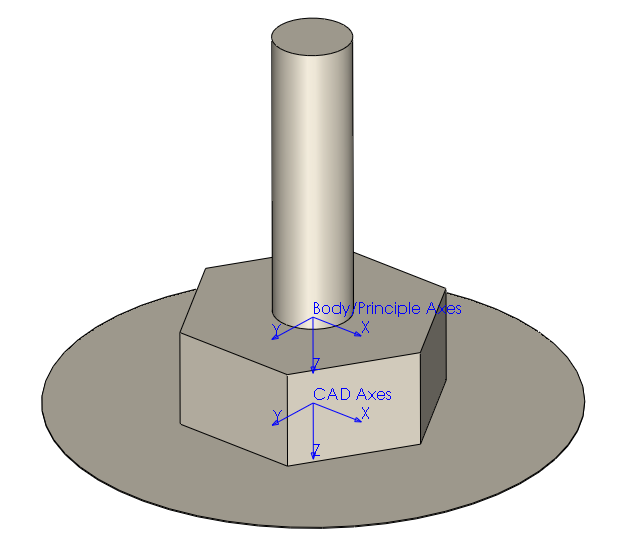
\includegraphics[scale=0.7]{Images/WMAP_CAD4.PNG}
\caption{A 3D model of the simplified satellite geometry. The body and principal axes are labeled and located at the spacecraft center of mass.}
\label{CAD model with frames}
\end{figure}


\begin{equation}
\vec{M} = \vec{I} \cdot \vec{\dot{\omega}}\ + \vec{\omega} \times \vec{I} \cdot \vec{\omega} \\ 
\end{equation}   



\begin{eqnarray}
M_x = I_{xx} \dot{\omega_x} + (I_{zz} - I_{yy})\omega_y \omega_z \nonumber \\
M_y = I_{yy} \dot{\omega_y} + (I_{xx} - I_{zz})\omega_z \omega_x \\
M_z = I_{zz} \dot{\omega_z} + (I_{yy} - I_{xx})\omega_x \omega_y \nonumber
\end{eqnarray}

\begin{equation}
I_{B} =
\begin{bmatrix} 
I_{xx} & I_{xy} & I_{xz} \\
I_{yx} & I_{yy} & I_{yz} \\ 
I_{zx} & I_{zy} & I_{zz} \\
\end{bmatrix}
=
\begin{bmatrix}
1005.5 & 0 & 0 \\
0 & 1005.5 & 0 \\ 
0 & 0 & 543.7
\end{bmatrix}
[kg/m^2].
\end{equation}

\begin{lstlisting}
function L_loc = LagrangePoints(mu)
%For a given value of mu, this function computes the location
%of all five Lagrange points for the circular restricted three
%body problem.

%Compute the location of the libration points
    l = 1 - mu;

    L_loc = zeros(5,3);

    %L1
    p_L1 = [1, 2*(mu - l), l^2 - 4*l*mu + mu^2, 2*mu*l*(l - mu) + mu - l,...
        mu^2*l^2 + 2*(l^2 + mu^2), mu^3 - l^3];
    L1roots = roots(p_L1);
    L1 = 0;
    for i = 1:5
        if (L1roots(i) > -mu) & (L1roots(i) < l)
         L1 = L1roots(i);
        end
    end
    L_loc(1,1) = L1;

    %L2
    %L3
    %L4
    %L5
end
\end{lstlisting}
